\documentclass[13pt]{scrreprt}
\usepackage[utf8]{inputenc} % use utf8 file encoding for TeX sources
\usepackage[T1]{fontenc}    % avoid garbled Unicode text in pdf
\usepackage[german]{babel}  % german hyphenation, quotes, etc
\usepackage{hyperref}       % detailed hyperlink/pdf configuration
\usepackage{graphicx}       % provides com\dfrac{m}{Nenner}ands for including figures
\usepackage{csquotes}       % provides \enquote{} macro for "quotes"
\usepackage[nonumberlist]{glossaries}     % provides glossary commands
\usepackage{enumitem}
\usepackage[center]{caption}
\usepackage[export]{adjustbox}

\title{
	\includegraphics[scale=0.5,center]{OfficialLogo.png}
	\\
Entwurfsdokument
}
\author{\\ \\ \\ \\ Marijan Petričević, Christoph Hartmann, Clara Walendy,\\
	 Jakob Dräger, Julius Meißner}

\begin{document}
\maketitle

% Platzierung des Inhaltsverzeichnisses
\tableofcontents

\chapter{Klarstellung für das Pflichtenheft}

In Zusammenarbeit mit Prof. Böhm und Leander Kurscheidt sind folgende Berichtigungen des Pflichtenheftes zu beachten.
\newline

\subsection{Datenbank}
	\begin{itemize} [label={}]
	\item Die Datenbank ist austauschbar. Dadurch befinden sich in einer Datenbank nur Graphen mit gleicher Knotenanzahl.
	\item Die Anzahl der Kanten ist einstellbar. Dies wird erreicht indem der minimale und maximale Knotengrad vom Benutzer eingegeben wird.
	\item Duplikate von Graphen werden mithilfe des minimalen BFS Code erkannt und durch das DBMS verhindert.
	\end{itemize}
	
\subsection{Bearbeitung eines Graphen}
	\begin{itemize} [label={}]
    \item Geringfügige Änderungen an den Graphen bedeuten keine mehrfache Selektierung.
    
	'Geringfügige Änderung' bedeutet:
	\begin{itemize} [label={}]
	\item Es werden auf den Graphen nur wenige einzelne Aktionen durchgeführt.
	\end{itemize}
	'Einzelne Aktion' bedeutet:
	\begin{itemize} [label={}]
	\item Hinzufügen oder Entfernen einer einzelnen Kante oder Knoten.
	\end{itemize}
	\end{itemize}
\subsection{Definitionen zur Graphgenerierung}
    \begin{itemize} [label={}]
	\item Der nächst-dichtere Graph:
	\begin{itemize} [label={}]
	\item Durch Addition von 1 auf den minimalen BFS Code eines Graphen, lässt sich der nächst dichtere Graph generieren. Wenn die Eigenschaft des Zusammenhangs dadurch zerstört wird, wird diese Addition sukzessiv durchgeführt, bis der Graph zusammenhängend ist.
	\end{itemize}
	\end{itemize}
	
\subsection{Darstellung der Korrelationen}
	\begin{itemize} [label={}]
	\item Alle Korrelationen mit einem Korrelationskoeffizienten über dem Threshold werden in der dafür vorgesehenen Spalte angezeigt. Der Threshold ist vom Benutzer einstellbar.
	\item Alle Korrelationen können in einem Popup als Matrix dargestellt werden.
	\end{itemize}
	
\subsection{Filter}
	\begin{itemize} [label={}]
    \item Folgende, nichttriviale Filter werden in das Programm eingebunden:
	\begin{itemize} [label={}]
	\item Dichtere Graphen, aber gleich viele Farben
	\item Dichtere Graphen, aber weniger Farben
	\item Dichtere Graphen, aber mehr Farben
	\item Weniger dichte Graphen, aber gleich viele Farben
	\item Weniger dichte Graphen, aber weniger Farben
	\item Weniger dichte Graphen, aber mehr Farben
	\item Gleich dichte Graphen, aber gleich viele Farben
	\item Gleich dichte Graphen, aber weniger Farben
	\item Gleich dichte Graphen, aber mehr Farben
	\end{itemize}
	\end{itemize}
	
\subsection{Erweiterbarkeit}
    \begin{itemize} [label={}]
	\item Die Erweiterbarkeit des Programms soll durch ein extra Dokument (im Sinne einer Anleitung) vereinfacht werden.
	Dieses Dokument ermöglicht einem Programmierer, ohne vollständiges Verständnis des Codes, das Hinzufügen von Merkmalen und Graphengeneratoren zur Anwendung.
	\end{itemize}
	
\subsection{GUI}
	\begin{itemize} [label={}]
    \item Folgende Änderungen an der GUI sind zu beachten:
	\begin{itemize} [label={}]
	\item Die Dichte muss nicht auf eine Zahl heruntergebrochen werden, sie reicht als Werkzeug.
	\item Die Anzahl dichterer Graphen wird angezeigt.
	\item Es besteht die Möglichkeit den BFS Code zu einem Graph auszugeben.
	\end{itemize}
    \end{itemize}
    
\chapter{Einleitung}
Dieses Entwurfsdokument ist im Rahmen des Pflichtmoduls Praxis der Softwareentwicklung des Bachelor-Studiengangs Informatik am Karlsruher Institut für Technologie entstanden. Das Projekt wurde am Lehrstuhl für Systeme der Informationsverwaltung angeboten.
Das vorliegende Dokument ist das Produkt der Entwurfsphase. Es enthält Erläuterungen der getroffenen Entwurfsentscheidungen und ermöglicht mit Hilfe von Klassendiagrammen einen Überblick über den Entwurf.
In diesem Entwurfsdokument werden die Architektur und der Aufbau, die Pakete samt enthaltener Module und deren Klassen mit Methoden und Attributen erklärt.
\\ \\
Das Entwurfsdokument dient dabei als Grundlage zur Implementierung und spezifiziert alle Teilaspekte der Software.

\chapter{Anforderungsanalyse}
Die Software benötigt zunächst eine Datenbank, um die Datenbestände der Graphen persistent zu speichern. Zudem ist das Filtern auf einer Datenbank einfacher als vergleichbare Verfahren.
Der nächste Teil ist der Graphgenerator. Mit ihm sollen Graphen zufällig generiert und mit allen Merkmalen in der Datenbank gespeichert werden. Dies bedeutet, dass der Graphgenerator die Graphen zunächst an das Algorithmen-Modul weitergeben muss und anschließend berechneten Daten mit dem Repository in die Datenbank eingefügt werden.
Der letzte Teil der Anwendung ist die GUI, mit der Graphen optisch dargestellt, geringfügig bearbeitet und Merkmale bzw. Korrelationen der Merkmale verdeutlicht werden. Dazu muss die GUI eine Anbindung an die Datenbank haben, diese filtern und den ausgewählten Graphen mittels Knoten und Kanten darstellen.
Zudem werden die Merkmale und Korrelationen angezeigt. Hierfür müssen der GUI sowohl die Merkmale als auch die Korrelationskoeffizenten mitgeteilt werden.
Damit die einzelnen Komponenten miteinander interagieren können, wird ein Eventhandling System implementiert, damit es keine feste Bindung unter den Modulen gibt.

\chapter{Entwurfs Architektur}

\section{Architektur}
	Graphitty gliedert sich in zwei Teile: Eine Anwendung mit einer Benutzerschnittstelle und einem Hintergrundspeicher 		zum Abspeichern der generierten Graphen und der vom Nutzer eingestellten Filtereinstellungen. \\
	Die Anwendung wurde gem\"aß dem Model-View-ViewModel (MVVM) Entwurfsmusters entworfen, welches 			\"Ahnlichkeiten zu Model View Controller hat. Das MVVM Muster sorgt f\"ur eine klare Trennung von Darstellungs- 		und Anwendungslogik, wodurch die Anwendung leichter zu testen, warten und erweitern wird. Das MVVM 			Entwurfsmuster teilt die Anwendung in drei separate Pakete auf:
	\begin{itemize}
		\item View: Kapselt die Benutzeroberfläche und Benutzeroberflächenlogik.
		\item View Model: Kapselt den Darstellungszustand und die Darstellungslogik.
		\item Model: Kapselt die Anwendungslogik und Daten. \\
	\end{itemize}
	Um einen geregelten Zugriff auf die Datenbank in der Anwendung zu ermöglichen, kommen die Entwurfsmuster Unit of Work und Repository zum Einsatz. Diese Muster bilden eine Abstraktionsebene über der 	Datenbank. Eine genauere Beschreibung der Funktionsweise dieser, kann in den zugehörigen Klassenbeschreibungen nachgelesen werden.
	\newline 
	Die Zuordnung von persistenten Daten und Objekten wird durch objektrelationale Abbildung (ORM, object relational 		mapping) gewährleistet. Das ORM erfolgt durch das Entity Framework, welches von Microsoft entwickelt wurde. 	
		
\section{Komponenten der Architektur}
	Im Folgenden werden die Module des MVVM Musters, sowie die Rolle und das Zusammenspiel dieser näher 			beschrieben.
	\subsection{View}
	Die View ist ein visuelles Element (Fenster oder Bedienelement) welches die Anordnung und das Aussehen von 		Bedienelementen definiert. Sie besitzt einen Datenkontext, welcher eine Referenz zu ihrem ViewModel ist. In der 		Regel herrscht eine 1:1 Beziehung zwischen View und ViewModel. Die Bedienelemente der View sind gebunden mit 	den \"offentlichen Eigenschaften und Kommandos des ViewModels. Das ViewModel benachrichtigt die View über 		Zustands\"anderungen, die sich in Folge dessen aktualisiert. Des Weiteren kann sie Validierungsregeln nutzen, die 		den Anwender \"uber  fehlerhafte Eingaben informieren.
	\newline
	Bem.: Zum Anzeigen von Graphen kommt das Graphenframework "GraphX" (Apache Lizenz) zum Einsatz. Das 		Framework ist derzeit nicht kompatibel mit dem MVVM Muster, weshalb es an dieser Stelle zur Verletzung des 		Musters kommen kann.
	\subsection{View Model}
	Das ViewModel koordiniert Interaktionen in der View zu den benötigten Model Klassen. Es bereitet die Daten des 		Models so auf, dass diese einfach von der View konsumiert werden können. Es ist das Bindeglied zwischen den 		beiden Modulen.
	\newline
	Das ViewModel kapselt wie bereits erwähnt den Darstellungszustand und die Darstellungslogik. Der Zustand und die 	Logik werden einer View in Form von \"offentlichen Eigenschaften und Kommandos bereitgestellt, eine View 			entscheidet dann wie diese gerendert werden. Diese \"offentlichen Eigenschaften k\"onnen unter anderem ein Model 	miteinschließen. Ein Model wird der View entweder direkt zur Verf\"ugung gestellt oder durch das ViewModel vorher 	aufbereitet. Jegliche \"Anderungen des Zustandes werden der View mitgeteilt.
	\subsection{Model}
	Das Model kapselt die Anwendungslogik, die Anwendungsdaten, sowie das Management der Daten. Es beinhaltet 		auch eine 	Datenzugriffsschicht, die für das Erstellen, Aktualisieren, Lesen und L\"oschen von persistenten Daten 		sorgt. Dazu werden in der Anwendung das Unit of Work und Repository Muster verwendet. Des weiteren informiert 		das 	Model das ViewModel über fehlerhafte Daten und über \"Anderungen.
	\subsubsection{Unit of Work und Repository}
	Die Unit of Work verwaltet und kapselt den Zugriff auf den Datenbankkontext und die Repositories. Der 				Datenbankkontext ist eine Objektdatenbank die von einem ORM Framework, dem Entity Framework erstellt wird. Die 		Repositories ermöglichen den Zugriff auf einzelne Tabellen des Datenbankkontextes bzw. der Datenbank.
	\\
	\begin{center}	
	\includegraphics[width=0.7\textwidth, angle=0]{DatenbankER.jpg}  	
	\\
	ER-Diagramm
	\\
	\end{center}
	\begin{center}
	\includegraphics[width=0.8\textwidth, angle=0]{SystemArchitektur.pdf}  	
	\\
    Die MVVM Module und das Zusammenspiel
    \end{center}	
    

	\section{Modul Kommunikation}
	Dieses Diagramm stellt die Kommunikation (bzw. Interaktion) der einzelnen Module dar. Es gibt einen groben Überblick über die Funktionsweise. Die Bezeichner der Aktionen sind keine Commands/Funktionen.
	\\ \ 
	\\ \ 


	\includegraphics[scale=0.7, center]{ModuleCommunication.jpg}


	\chapter{Klassenbeschreibungen View}
	Die View ist hierarchisch aufgebaut, jeder View ist ein ViewModel zugeordnet. Das zugeordnete ViewModel ist eine Abstraktion der View. S\"amtliche \"offentlichen Attribute eines zugeordneten ViewModels stehen der View zur Verf\"ugung. Die View verwendet geeignete visuelle Elemente die Teil der Windows Presentation Foundation sind um diese Attribute visuell darzustellen. Die MainView ist ein Fenster und alle anderen Views sind UserControls. Da eine View in XAML implementiert wird, wird im folgenden keine genaue Klassenbeschreibung angegeben.
	\newline
	\includegraphics[angle=90, scale=0.3, center]{View.png}
	\section{MainView}
	Die MainView ist das Hauptfenster der Anwendung, alle anderen Views werden in diese View integriert.
	\section{FiltersView}
	Sie listet alle aktiven und verfügbaren Filter auf, die der Nutzer hinzuf\"ugen oder entfernen kann. Sie bietet zudem Schaltfl\"achen zum Speichern oder Laden von Filtereinstellungen an.
	\section{GraphsView}
	Sie listen alle Graphen die den aktiven Filterkriterien gen\"ugen. Der Nutzer kann aus der Liste Graphen selektieren.
	\section{PropertiesView}
	Hier werden die Merkmale eines in der GraphsView selektierten Graphen angezeigt.
	\newpage
	\section{GraphVisualizerView}
	Die GraphVisualizerView stellt einen in der GraphsView selektierten Graphen visuell dar. Hier kann der Nutzer auch mithilfe von Schaltfl\"achen den Graphen editieren. Die genauere Funktionalit\"at zu dieser Klasse ist im GraphVisualizerViewModel.
	\begin{itemize}[label = {$\circ$}]
		\item {\large \textbf{\textit{Attribute}}\par}
		\begin{description}
			\item [private GraphVisualizerViewModel vm] \hfill \\ Eine Referenz zum ViewModel um den Datacontext zu setzen und Commands zu senden.
		\end{description}
		\item {\large \textbf{\textit{Konstruktoren}}\par}
		\begin{description}
			\item [public MainWindow()] \hfill \\ Initialisiert die View und setzt den Datacontext auf das GraphVisualizerViewModel
		\end{description}
	\end{itemize}
	
	\section{GeneratorView}
	In der GeneratorView werdem dem Nutzer Selektions- und Eingabefl\"achen angeboten um einen Generator zu konfigurieren. Diese View beinhaltet DataTemplates f\"ur Klassen, die die Interfaces IVertexFactoryViewModel bzw. IEdgeFactoryViewModel implementieren. Diese DataTemplates bieten weitere Generator-Konfigurationsm\"oglichkeiten. Zudem gibt es im der GeneratorView Schaltfl\"achen um die Generierung zu starten oder eine Laufende zu stoppen.
	\section{ConsoleView}
	Sie stellt den aktuellen Log in textueller Form dar.
	\section{CorrelationsTableView}
	Sie listet die am st\"arksten korrellierenden Merkmale der Graphendatenbank auf. Der Nutzer hat eine M\"oglichkeit den mindest-Korrelationskoeffizienten selbst zu setzen, sowie eine Schaltfl\"ache um sich eine Matrix anzeigen zu lassen.
	
	\chapter{Klassenbeschreibungen ViewModel}
	Das ViewModel Paket ist hierarchisch aufgebaut, wobei das MainViewModel die Wurzel der Hierarchie ist. Alle anderen ViewModels sind Kinder des MainViewModels. Gerechtfertigt wird diese Hierarchie durch die ebenfalls hierarchisch aufgebaute View. 
	\newline
	Die Kommunikation zwischen den ViewModels auf derselben Ebene wird durch das Publish-Subscribe Muster geregelt. ViewModels k\"onnen Ereignisse abonnieren oder ver\"offentlichen. Ein Aggregator wird verwendet um Publisher und Subscriber voneinander loszukoppeln. Publisher ver\"offentlichen Ereignisse \"uber den Aggregator. Subscriber abonnieren den Aggregator. Dadurch muss keiner der Publisher Kenntnisse \"uber die Subscriber haben. 
	\newline
	Zudem erweitert jedes ViewModel die BindableBase eine abstrakte Klasse, welche eine Implementierung zur Verf\"ugung stellt, die das Bindungssystem der Windows Presentation Foundation \"uber \"Anderungen des jeweiligen ViewModels benachrichtigt. Die BindableBase implementiert das INotifyPropertyChanged Interface.
	\newline
	ViewModels, die ein ICommand \"offentlich bereitstellen verwenden das Kommando Entwurfsmuster. Das Befehlsobjekt wird im Konstruktor der ViewModels instanziiert und dem \"offentlichen ICommand zugewiesen.
	\newpage
	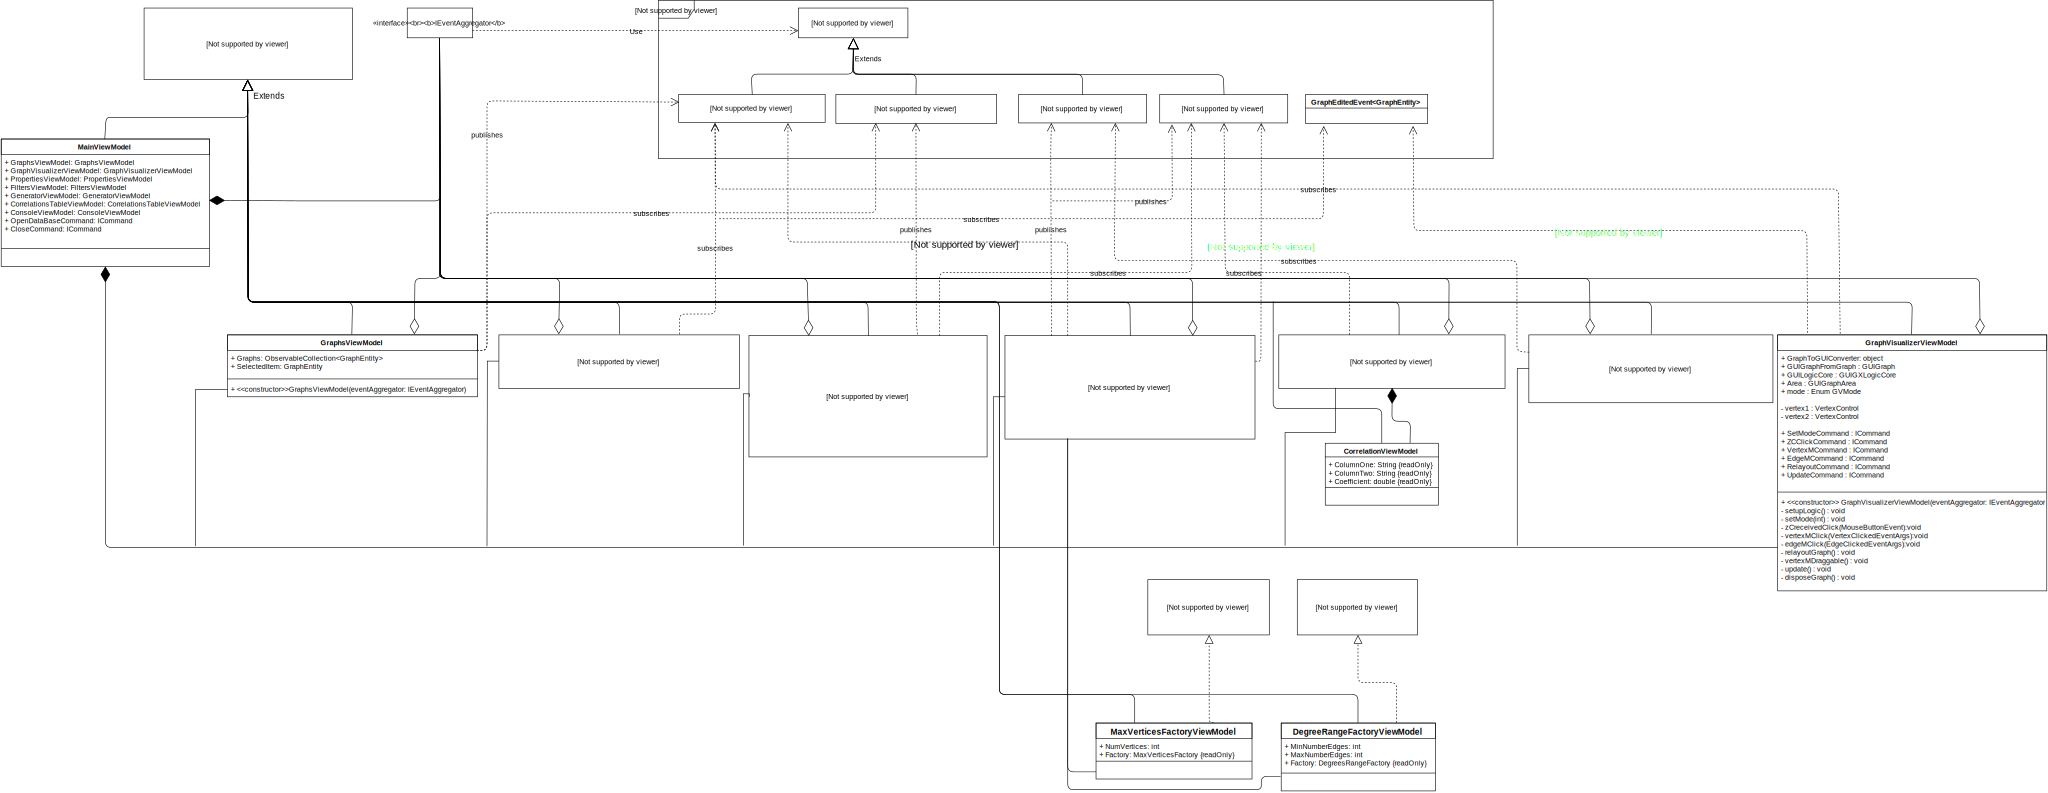
\includegraphics[angle=90, scale=0.2, center]{ViewModel.png}
	\section{MainViewModel}
	Dieses ViewModel ist die Wurzel in der Hierarchie der ViewModels. Es instanziiert s\"amtliche Kinder und einen EventAggregator, der den Kindern zur Kommunikation bereitgestellt wird. Jedes der Kinder wird \"uber \"offentliche Eigenschaften verf\"ugbar gemacht, sodass die MainView diese konsumieren kann.
	\begin{itemize}[label = {$\circ$}]
		\item {\large \textbf{\textit{Attribute}}\par}
		\begin{description}
			\item [+ GraphsViewModel: GraphsViewModel] \hfill
			\item [+ GraphVisualizerViewModel: GraphVisualizerViewModel] \hfill
			\item [+ PropertiesViewModel: PropertiesViewModel] \hfill
			\item [+ FiltersViewModel: FiltersViewModel] \hfill
			\item [+ GeneratorViewModel: GeneratorViewModel] \hfill
			\item [+ CorrelationsTableViewModel: CorrelationsTableViewModel] \hfill
			\item [+ ConsoleViewModel: ConsoleViewModel] \hfill
			\item [+ OpenDataBaseCommand: ICommand]\hfill \\ \"Offnet ein neues Fenster, in dem der Benutzer eine Verbindung zu einer Datenbank herstellen kann.
			\item [+ CloseCommand: ICommand]\hfill \\ Sorgt f\"ur eine sordnungsgem\"aße Terminierung des Programmes.
		\end{description}
	\end{itemize}
	\newpage
	\section{FiltersViewModel}
	Das FiltersViewModel ver\"offentlicht Ereignisse vom Typ \\FilterAppliedEvent<List<GraphEntity>>, nachdem sich die aktiven Filter ver\"andern. Es bietet einer View verschiedene Sammlungen von Filtern an und f\"ur die einzelnen Filter werden Kommandos zum entfernen oder hinzuf\"ugen dieser bereitgestellt. Zudem k\"onnen mit diesem ViewModel Filtereinstellungen gespeichert oder geladen werden. Zudem ist das ViewModel auch ein Subscriber des DatabaseChangedEvent<Object>, wenn es zu einer Aktualisierung der Datenbankeintr\"age kommt, m\"ussen die Filter erneut angewandt werden.
	\begin{itemize}[label = {$\circ$}]
		\item {\large \textbf{\textit{Attribute}}\par}
		\begin{description}
			\item [+ ActiveFilters: ObservableCollection<IFilter>] \hfill \\Dies sind die aktiven Filter.
			\item [+ GeneralFilters: ObservableCollection<IFilter>] \hfill \\ Dies sind zur Verf\"ugung stehende Filter, die generelle Eigenschaften eines Graphen betreffen.
			\item [+ TotalColoringFilters: ObservableCollection<IFilter>] \hfill \\Dies sind zur Verf\"ugung stehende Filter, die die Totalf\"arbungseigenschaften eines Graphen betreffen.
			\item [+ AddFilterCommand: ICommand] \hfill \\ Dieses Kommando aktiviert einen Filter.
			\item [+ RemoveFilterCommand: ICommand] \hfill \\ Dieses Kommando deaktiviert einen Filter.
			\item [+ SaveFilterCommand: ICommand] \hfill \\ Speichert die aktuelle Filterauswahl.
			\item [+ LoadFilterCommand: ICommand] \hfill \\ L\"adt eine fr\"uher abgespeicherte Filterauswahl.
		\end{description}
		\item {\large \textbf{\textit{Konstruktoren}}\par}
		\begin{description}
			\item [+  FiltersViewModel(eventAggregator: IEventAggregator)] \hfill \\ Der Konstruktor nimmt einen Event Aggregator als Parameter entgegen, über welchen dieses ViewModel Ereignisse ver\"offentlichen und empfangen kann.
		\end{description}
	\end{itemize}
	
	\section{GraphsViewModel}
	Das GraphsViewModel abonniert Ereignisse vom Typ FilterAppliedEvent<List<GraphEntity>>. Nach Erhalt dieses Ereignisses beinhaltet es die aktuell gefilterten Graphen als Sammlung. Zudem ist es selbst Publisher von Ereignissen des Typs SelectionChangedEvent<GraphEntity>, dass immer dann ver\"offentlicht wird, wenn sich der aktuell ausgew\"ahlte Graph \"andert.
	\begin{itemize}[label = {$\circ$}]
		\item {\large \textbf{\textit{Attribute}}\par}
		\begin{description}
			\item [+ Graphs: ObservableCollection<GraphEntity>] \hfill \\Dies sind die aktuell durch den Filter festgelegten Graphen.
			\item [+ SelectedItem: GraphEntity] \hfill \\ Der aktuell selektierte Graph der Graphs ObservableCollection.
		\end{description}
		\item {\large \textbf{\textit{Konstruktoren}}\par}
		\begin{description}
			\item [+ GraphsViewModel(eventAggregator: IEventAggregator)] \hfill \\ Der Konstruktor nimmt einen Event Aggregator als Parameter entgegen, über welchen dieses ViewModel Ereignisse empfangen und ver\"offentlichen kann.
		\end{description}
	\end{itemize}
	\newpage
	\section{PropertiesViewModel}
	Das PropertiesViewModel abonniert Ereignisse vom Typ SelectionChangedEvent<GraphEntity> und GraphEditedEvent<GraphEntity>, dadurch erh\"alt es immerzu den aktuell selektierten Graphen des GraphsViewModels oder den bearbeiteten Graphen vom GraphVisualizerViewModel. Das PropertiesViewModel stellt dann diesen Graphen der konsumierenden PropertiesView zur Verf\"ugung, die die Eigenschaften des Graphen anzeigt.
	\begin{itemize}[label = {$\circ$}]
		\item {\large \textbf{\textit{Attribute}}\par}
		\begin{description}
			\item [+ Graph : GraphEntity] \hfill \\Der aktuell selektierte Graph. Eine View hat Zugriff auf s\"amtliche Eigenschaften.
		\end{description}
		\item {\large \textbf{\textit{Konstruktoren}}\par}
		\begin{description}
			\item [+ GraphsViewModel(eventAggregator: IEventAggregator] \hfill \\ Der Konstruktor nimmt einen Event Aggregator als Parameter entgegen, über welchen dieses ViewModel Ereignisse abonnieren kann.
		\end{description}
	\end{itemize}
	
	\section{GraphVisualizerViewModel}
	Das GraphVisualizerViewModel (GVVM) ist der Datenkontext für die GraphVisualizerView. Das GVVM h\"alt alle Daten und Datenoperationen für die Graphendarstellung. Es abonniert Ereignisse vom Typ SelectionChangedEvent<GraphEntity>, dadurch erh\"alt es immerzu den aktuell selektierten Graphen. Zudem ver\"offentlicht es Ereignisse des Typs GraphEditedEvent<GraphEntity> um anderen ViewModels \"anderungen am Graphen bekannt zu machen.
	\newpage
	\begin{itemize}[label = {$\circ$}]
		\item {\large \textbf{\textit{Attribute}}\par}
		\begin{description}
			\item [+ Area : GUIGraphArea] \hfill \\ Die Klasse dient zur Darstellung des Graphen und muss zum Bearbeiten referenziert werden
			\item [+ Mode : Enum GVMode] \hfill \\ Eine einfache Statemachine, die Funktionen zur Bearbeitung voneinander trennt
			\item [+ SetModeCommand: ICommand]\hfill \\ Ändert den Modus des VM. Modi steuern die verfügbaren Funktionen
			\item [+ ZCClickCommand: ICommand]\hfill \\ Leitet Klicks auf die leere Fl\"ache weiter
			\item [+ VertexMCommand: ICommand]\hfill \\ Leitet Klicks auf Vertices weiter
			\item [+ EdgeMCommand: ICommand]\hfill \\ Leitet Klicks auf Edges weiter
			\item [+ RelayoutCommand: ICommand]\hfill \\ Stößt ein Relayout des Graphs an
			\item [+ UpdateCommand: ICommand]\hfill \\ Stößt ein Update der Area an
			\item [- vertex1 : VertexControl] \hfill \\ VertexControl Referenz zur Edge-Erstellung
			\item [- vertex2 : VertexControl] \hfill \\ VertexControl Referenz zur Edge-Erstellung
			\item [- guiGraphFromGraph : GUIGraph] \hfill \\ Der konvertierte GUIGraph vom anzuzeigenden Graph
			\item [- guiLogicCore : GUIGXLogicCore] \hfill \\ Die Klasse stellt Layout- und Routing-Algorithmen zur Verfügung
		\end{description}
		\item {\large \textbf{\textit{Konstruktoren}}\par}
		\begin{description}
			\item [+ GraphVisualizerViewModel(pArea : GUIGraphArea)] \hfill \\ Initialisiert das ViewModel mit den Default-Werten und setzt die Referenz auf das Area-Objekt
		\end{description}
		\item {\large \textbf{\textit{Methoden}}\par}
		\begin{description}
			\item [- setMode(int) : void] \hfill \\ Methode zum ändern der Statemachine
			\item [- zCreceivedClick(Args : MouseButtonEventArgs) : void] \hfill \\ Behandelt Klicks ohne spezifisches Ziel
			\item [- vertexMClick(Args : VertexClickedEventArgs) : void] \hfill \\ Behandelt Klicks auf Vertices
			\item [- edgeMClick(Args : EdgeClickedEventArgs) : void] \hfill \\ Behandelt Klicks auf Edges
			\item [- vertexMDraggable() : void] \hfill \\ Erlaubt das verschieben von Vertices
			\item [- relayoutGraph() : void] \hfill \\ Berechnet ein neues Layout des Graphs
			\item [- update() : void] \hfill \\ Updated den Datagraph im Hintergrund und zeichnet den Graphen neu
			\item [- setupLogic() : void] \hfill \\ Setup-Methode für das GUILogicCore-Objekt. Setzt Layouttyp und Layoutparameter
			\item [- disposeGraph() : void] \hfill \\ Entfernt den aktuellen Graph sicher aus der GUI
			\item [- convertGraph(GraphToConvert : Graph) : GUIGraph] \hfill \\ Convertiert ein Graph-Objekt in ein darstellbares GUIGraph-Objekt
		\end{description}
	\end{itemize}
	\newpage
	\section{GeneratorViewModel}
	Das GeneratorViewModel ver\"offentlicht Ereignisse vom Typ WriteLogEvent<String>, dies sind Ereignisse mit textuellen Informationen \"uber aktuelle Vorg\"ange im Generator. Es ver\"offentlicht auch Ereignisse vom Typ DatabaseChangedEvent<object> um andere ViewModels \"uber neu generierte Graphen zu informieren.
Das ViewModel stellt einer View Eigenschaften zur Verf\"ugung, die die Generierungseinstellungen konfigurieren. Es bietet zudem Kommandos an, die eine Generierung von Graphen veranlassen.
	\begin{itemize}[label = {$\circ$}]
		\item {\large \textbf{\textit{Attribute}}\par}
		\begin{description}
			\item [+ NumberOfGraphs: int] \hfill \\ Die Anzahl der 	zu generierenden Graphen.
			\item [+ GenerateTuple: bool] \hfill \\ Wahr, falls zus\"atzlich zu jedem generierten Graphen der n\"achst dichtere berechnet werden soll.
			\item [+ SelectedGraphConsequentiveNextDennser: bool] \hfill \\ Wahr, falls vom aktuell selektierten Graphen immerzu der n\"achst dichtere Graph berechnet werden soll. 
			\item [+ SelectedGraphGenerateNextDenser: bool] \hfill \\ Wahr, falls einmalig der n\"achst dichtere Graph berechnet werden soll.
			\item [+ Generating: bool \{readOnly\}] \hfill \\ Wahr, falls aktuell Graphen generiert werden.
			\item [+ GenerateCommand: ICommand] \hfill \\ Startet die Graphengenerierung.
		\end{description}
		\item {\large \textbf{\textit{Konstruktoren}}\par}
		\begin{description}
			\item [+  GeneratorViewModel(eventAggregator: IEventAggregator)] \hfill \\ Der Konstruktor nimmt einen Event Aggregator als Parameter entgegen, über welchen dieses ViewModel Ereignisse ver\"offentlichen kann.
		\end{description}
	\end{itemize}
	
	\section{IVertexFactoryViewModel}
	\begin{itemize}[label = {$\circ$}]
		\item {\large \textbf{\textit{Attribute}}\par}
		\begin{description}
			\item [+ DisplayName: String \{readOnly\}] \hfill \\ Der Anzeigename.
			\item [+ Factory: IVertexFactory \{readOnly\}] \hfill \\ Das Model, welches durch das ViewModel repr\"asentiert wird.	
		\end{description}
	\end{itemize}
	
	\section{IEdgeFactoryViewModel}
	\begin{itemize}[label = {$\circ$}]
		\item {\large \textbf{\textit{Attribute}}\par}
		\begin{description}
			\item [+ DisplayName: String \{readOnlyß\}] \hfill \\ Der Anzeigename.
			\item [+ Factory: IEdgeFactory \{readOnly\}] \hfill \\ Das Model, welches durch das ViewModel repr\"asentiert wird.	
		\end{description}
	\end{itemize}

	\section{MaxVerticesFactoryViewModel}
	Implementiert das IVertexFactoryViewModel Interface. Es bietet einem Daten-Template Attribute an, sodass die maximale Anzahl der zu generierenden Graphen festlegt werden kann.
	\begin{itemize}[label = {$\circ$}]
		\item {\large \textbf{\textit{Attribute}}\par}
		\begin{description}
			\item [+ NumVertices: int] \hfill \\ Die festlegbare Anzahl.
			\item [+ Factory: MaxVerticesFactory \{readOnly\}] \hfill \\ Schr\"ankt das Model ein vom Typen MaxVerticesFactory zu sein.			
		\end{description}
	\end{itemize}
	\newpage
	\section{DegreeRangeFactoryViewModel}
	Implementiert das IEdgeFactoryViewModel Interface. Es bietet einem Daten-Template Attribute an, sodass ein Bereich f\"ur die Anzahl der Kanten festgelegt werden kann.
	\begin{itemize}[label = {$\circ$}]
		\item {\large \textbf{\textit{Attribute}}\par}
		\begin{description}
			\item [+ MinNumberEdges: int] \hfill \\ Die festlegbare Anzahl.
			\item [+ MaxNumberEdges: int] \hfill \\ Die festlegbare Anzahl.
			\item [+ Factory: DegreesRangeFactory \{readOnly\}] \hfill \\ Schr\"ankt das Model ein vom Typen DegreesRangeFactory zu sein.			
		\end{description}
	\end{itemize}

	
	\section{ConsoleViewModel}
	Das ConsoleViewModel abonniert Ereignisse vom Typ WriteLogEvent<string>, dadurch erh\"alt es textuelle Informationen, die in eine Log-Datei geschrieben werden. Das ViewModel stellt diesen Log in form eines Strings der ConsoleView zur Verf\"ugung.
	\begin{itemize}[label = {$\circ$}]
		\item {\large \textbf{\textit{Attribute}}\par}
		\begin{description}
			\item [+ TextLog: String \{readOnly\}] \hfill \\ Der aktuelle Log-Text aus einer Log-Datei.
		\end{description}
		\item {\large \textbf{\textit{Konstruktoren}}\par}
		\begin{description}
			\item [+  ConsoleViewModel(eventAggregator: IEventAggregator)] \hfill \\ Der Konstruktor nimmt einen Event Aggregator als Parameter entgegen, über welchen dieses ViewModel Ereignisse abonnieren kann.
		\end{description}
	\end{itemize}
	\newpage
	\section{CorrelationsTableViewModel}
	Das CorrelationsViewModel stellt die Pearson-Korrelationskoeffizienten von Grapheneigenschaften in Form einer Sammlung zur Verf\"ugung und bietet eine M\"oglichkeit diese darzustellen. Es abbonniert Ereignisse vom Typ DatabaseChangedEvent<object> um die Korrelationswerte zu aktualisieren.
	\begin{itemize}[label = {$\circ$}]
		\item {\large \textbf{\textit{Attribute}}\par}
		\begin{description}
			\item [+ Correlations: ObservableCollection<CorrelationViewModel>] \hfill \\ Eine Sammlung von Korrelationskoeffizienten mit den jeweiligen Eigenschaftsbezeichnungen.
			\item [+ ShowMatrixCommand: ICommand] \hfill \\ Zeigt die gesamte Matrix mit den Koeffizienten an.
		\end{description}
		\item {\large \textbf{\textit{Konstruktoren}}\par}
		\begin{description}
			\item [+ CorrelationsTableViewModel(eveAgg : IEventAggregator)] \hfill \\ Der Konstruktor nimmt einen Event Aggregator als Parameter entgegen, über welchen dieses ViewModel Ereignisse abonnieren kann.
		\end{description}
	\end{itemize}
	
	\section{CorrelationViewModel}
	Stellt den Namen der Spalten, sowie einen Koeffizienten einem Daten-Template zur Verf\"ugung. Es wird dazu verwendet eine Korrelation leichter zug\"anglich f\"ur ein Daten-Template zu machen.
	\begin{itemize}[label = {$\circ$}]
		\item {\large \textbf{\textit{Attribute}}\par}
		\begin{description}
			\item [+ ColumnOne: String \{readOnly\}] \hfill \\ Bezeichnung der ersten Spalte.
			\item [+ ColumnTwo: String \{readOnly\}] \hfill \\ Bezeichnung der zweiten Spalte.
			\item [+ Coefficient: double \{readOnly\}] \hfill \\ Pearson-Korrelationskoeffizient der beiden Spalten.
		\end{description}
		\item {\large \textbf{\textit{Konstruktoren}}\par}
		\begin{description}
			\item [+  CorrelationViewModel()] \hfill \\ Standardkonstruktor
		\end{description}
	\end{itemize}
	
	\section{Modul Events}
	Dieses Modul beinhaltet alle Events, die zur Kommunikation zwischen ViewModels mittels des Publish-Subscribe Musters verwendet werden. Diese Events erweitern alle die Klasse PubSubEvent<TPayload>, welche vom Prism.WPF Framework zur Verf\"ugung gestellt wird.
	
	\subsection{SelectionChangedEvent<GraphEntity>}
	Dieses Event wird bei der \"Anderung der Auswahl eines Graphen ausgel\"ost. Dabei wird der selektierte Graph als Event-Parameter \"ubergeben.
	\subsection {FilterAppliedEvent<List<GraphEntity> >}
	Dieses Event wird bei jeder Aktivierung oder Deaktivierung eines Filters ausgel\"ost. Als Event-Parameter wird eine Liste von Graphen \"ubergeben, die diesen Filterkriterien entsprechen.
	\subsection{WriteLogEvent<String>}
	Dieses Event wird immer dann ausgel\"ost, wenn ein Text an das ConsoleViewModel gereicht werden muss, der den Text in den Log eintr\"agt. Als Event-Parameter wird der zu schreibende Text \"ubergeben.
	\subsection{DatabaseChangedEvent<object>}
	Dieses Event wird immer dann ausgel\"ost, wenn sich Eintr\"age in der Datenbank \"andern.
	\subsection{GraphEditedEvent<GraphEntity>}
	Dieses Event wird immer dann ausgel\"ost, wenn ein selektierter Graph bearbeitet wurde. Der bearbeitete Graph wird als Last mit\"ubergeben.
	
	\chapter{Klassenbeschreibungen Model}
	Das Model wird in einzelne Module aufgeteilt. Diese werden im Folgenden im Detail beschrieben.
	
	\section{Modul Data Access Layer}
	Dieses Modul beinhaltet s\"amtliche Klassen, die notwendig sind um auf die Datenbank zuzugreifen. Das Modul verwendet das Data Access Object Muster, welches sich in der Klasse Graphitty Context wiederspiegelt. Zudem verwendet das Modul das Unit Of Work und Repository Muster. Damit ist das gesamte Modul eine Abstraktionsebene zwischen der Anwendungslogik und dem Datenbankzugriff. Die Muster isolieren die Anwendung von \"Anderungen in der unterliegenden Datenschicht und erleichtern das Testen aller Komponenten, die einen Zugriff auf persistente Daten ben\"otigen.
	\newline
	\includegraphics[scale=0.4, center]{DataAccessLayer.png}
	\subsection{GraphittyContext}
	Dies ist die Objektdatenbank, die das EntityFramework verwendet um eine passende Migration einer relationalen MariaDB Datenbank zu erstellen.
	\begin{itemize}[label = {$\circ$}]
		\item {\large \textbf{\textit{Attribute}}\par}
		\begin{description}
			\item [+ Graphs: DbSet<GraphEntity>] \hfill \\ Repr\"asentiert die Tabelle der Graphen in der Datenbank.
			\item [+ Filters: DbSet<FilterEntity>] \hfill \\ Repr\"asentiert die Tabelle der Filter in der Datenbank.
		\end{description}
		\item {\large \textbf{\textit{Vererbung}}\par}
		\begin{description}
			\item [DbContext] \hfill \\ Teil des Entity Frameworks.
		\end{description}
	\end{itemize}
	
	\subsection{UnitOfWork}	
	Die Unit Of Work ist ein Singelton. Sie bietet Zugriff auf alle Repositories und stellt diesen einen einheitlichen Datenbankkontext zur Verf\"ugung.
	\begin{itemize}[label = {$\circ$}]
		\item {\large \textbf{\textit{Interfaces}}\par}
		\begin{description}
			\item [IDisposeable] \hfill \\ Diese Schnittstelle stellt einen Mechanismus zum Freigeben nicht verwalteter Ressourcen bereit.
		\end{description}
		\item {\large \textbf{\textit{Attribute}}\par}
		\begin{description}
			\item [+ GraphRepostitory: Repository<GraphEntity>] \hfill \\ Ist ein Beh\"alter der Zugriff auf Objekte vom Typen GraphEntity erm\"oglicht.		
			\item [+ FilterRepository: Repository<FilterEntity>] \hfill \\ Ist ein Beh\"alter der Zugriff auf Objekte vom Typen GraphEntity erm\"oglicht.
			\item [+ Instance: UnitOfWork] \hfill \\ Ein statisches Attribut. Es bietet Zugriff auf die Instanz des Singletons.
		\end{description}
		\item {\large \textbf{\textit{Konstruktoren}}\par}
		\begin{description}
			\item [-  UnitOfWork()] \hfill \\ Ist der private Konstruktor um dem Singleton Muster gerecht zu werden.
		\end{description}
		\item {\large \textbf{\textit{Methoden}}\par}
		\begin{description}
			\item [+ Save()] \hfill \\ Speichert \"Anderungen in der Datenbank ab.
			\item [+ Dispose()] \hfill \\ Verwirft den Kontext und trennt die Verbindung zur Datenbank.
		\end{description}
	\end{itemize}
	
	\subsection{Repository<TEntity>}	
	Ist ein generischer Beh\"alter, der verschiedene Create-Read-Update-Delete (CRUD) Methoden anbietet, mit denen Objekte vom Typ TEntity verwaltet werden k\"onnen.
	\begin{itemize}[label = {$\circ$}]
	\item {\large\textbf{\textit{Konstruktoren}}\par}
		\begin{description}
			\item [+ Repository(context: DbContext)] \hfill \\ Der Konstruktor nimmt eine Referenz auf den Datenbankkontext entgegen.
		\end{description}
	\item {\large \textbf{\textit{Methoden}}\par}
		\begin{description}
			\item [+ Create(entity: TEntity): void] \hfill \\ Erstellt einen neuen Eintrag in der Datenbank f\"ur das \"ubergebene Objekt.
			\item [+ Update(entity: TEntity): void] \hfill \\ Aktualisiert den Eintrag in der Datenbank f\"ur das \"ubergebene Objekt.
			\item [+ Delete(id: object): void] \hfill \\ L\"oscht den Eintrag mit der \"ubergebenen ID aus der Datenbank.
			\item [+ Delete(entity: TEntity): void] \hfill \\ L\"oscht den Eintrag aus der Datenbank f\"ur das \"ubergebene Objekt.
			\item [+ GetAll(orderBy: (IQueryable<TEntity> -> IOrderedQueryable<TEntity>),]
			\item[skip : int, take:int): IEnumerable<TEntity>] \hfill \\ Gibt alle Objekte vom Typ TEntity zur\"uck und ordnet diese gem\"aß der Lambdafunktion orderBy, \"uberspringt ggfs. n Objekte, nimmt ggfs. k Objekte. Alle Parameter sind optional und haben einen default Wert der keine Auswirkung hat.
			\item [+ Get(filter: (TEntity -> bool), ]
			\item [orderBy:(IQueryable<TEntity> -> IOrderedQueryable<TEntity>),]
			\item [skip: int, take: int): IEnumerable<TEntity>] \hfill \\ Holt alle Eintr\"age aus der Datenbank die dem Filter entsprechen, ordnet diese ggfs., \"uberspringt ggfs. n Objekte, nimmt ggfs. k Objekte. Alle Parameter sind optional und haben einen default Wert der keine Auswirkung hat.
			\item [+ GetOne(filter: (TEntity -> bool)): TEntity] \hfill \\ Holt irgendein Objekt das dem Filter gerecht wird aus der Datenbank.
			\item [+ GetById(id: object): TEntity] \hfill \\ Holt einen Eintrag mit der gegebenen ID aus der Datenbank.
			\item [+ GetCount(filter: (TEntity -> bool)): int] \hfill \\ Gibt die Anzahl der Eintr\"age, die dem Filter gerecht werden zur\"uck.
			\item [+ Exists(filter: (TEntity -> bool)): bool] \hfill \\ Pr\"uft ob ein Objekt, das dem Filter gerecht wird in der Datenbank existiert.
		\end{description}
	\end{itemize}
	
	\section{Modul Graph}
	
	\includegraphics[scale=0.9, center]{GraphPackage.jpg}
	
	\subsection{Klasse GraphEntity}
	Die Klasse GraphEntity gibt die Struktur für die Speicherung in der Datenbank vor, welche dann durch das Entity-Framework umgesetzt wird.
	\begin{itemize}[label = {$\circ$}]
		\item {\large \textbf{\textit{Attribute}}\par}
		\begin{description}
			\item [+ ID: int] \hfill \\ ID zur Identifikation eines Graphens.
			\item [+ NumVertices: int] \hfill \\ Anzahl der Knoten im Graph.
			\item [+ NumEdges: int] \hfill \\ Anzahl der Kanten im Graph.
			\item [+ IsTotallyColorable: bool] \hfill \\ Ist die Totalf\"arbungsvermutung erfüllt.
			\item [+ BFSCode: String] \hfill \\ Der BFS-Code des Graphen.
			\item [+ BFSDensity: int] \hfill \\ Die BFS-Dichte des Graphen.
			\item [+ AverageVertexDegree: int] \hfill \\ Durchschnittlicher Knotengrad.
			\item [+ MaxVertexDegree: int] \hfill \\Maximaler Knotengrad.
			\item [+ LargestCliqueSize: int] \hfill \\ Größe der größten Clique im Graph.
			\item [+ NumCliquesOfSizeK: int] \hfill \\ Anzahl der Cliquen der Größe k.
			\item [+ NumDenserGraphsBFS: int] \hfill \\ Anzahl der nach BFS-Code dichteren Graphen.
			\item [+ Profil: String] \hfill \\ Profil des Graphen.
			\item [+ NumDenserGraphsProfile: int] \hfill \\ Anzahl der nach Profil dichteren Graphen.
			\item [+ TotalChromaticNumber: int] \hfill \\ die totalchromatische Zahl des Graphen.
			\item [+ MinimalColoringComplexityInSeconds: int] \hfill \\ Aufwand in Sekunden um eine gültige Totalfärbung zu finden.
			\item [+ NumGraphsWithSmallerEqualChromaticNumber: int] \hfill \\ Anzahl der Graphen mit einer kleiner/gleichen totalchromatischen Zahl.
			\item [+ NumDifferentTotalColorings: int] \hfill \\ Anzahl der unterschiedlichen Totalfärbungen.
		\end{description}
	\end{itemize}
	
	\subsection{Klasse Graph}
	Die Klasse Graph stellt einen Graphen dar.
	\begin{itemize}[label = {$\circ$}]
		\item {\large \textbf{\textit{Vererbung}}\par}
		\begin{description}
			\item [GraphEntity] \hfill \\ Graph erbt von der Klasse GraphEntity.
		\end{description}
		\item {\large \textbf{\textit{Attribute}}\par}
		\begin{description}
			\item [+ Vertices: List<Vertex>] \hfill \\Liste der Knoten des Graphen.
			\item [+ Edges: List<Edge>] \hfill \\Liste der Kanten des Graphen.
		\end{description}
		\item {\large \textbf{\textit{Konstruktoren}}\par}
		\begin{description}
			\item [+ Graph()] \hfill \\ Standartkonstruktor.
			\item [+ Graph(vertices: List<Vertex>, edges: List<Edge>)] \hfill  \\ Erzeugt einen Graphen mit Knoten und Kanten aus den übergebenen Listen.
		\end{description}
	\newpage
		\item {\large \textbf{\textit{Methoden}}\par}
		\begin{description}
			\item [+ Compare(graph: Graph): bool] \hfill \\ Vergleicht den Graphen mit einem übergebenen Graphen. Falls die Kanten und Knoten gleich sind, wird true zurückgegeben.
			\item [+ CompareBFS(graph: Graph): int] \hfill \\ Vergleicht den BFS-Code des Graphen mit einem übergebenen. Ist der übergebene Graph nach BFS dichter, wird 1 zurückgegeben. Ist er weniger dicht, wird -1 zurückgegeben. Bei Gleichheit 0.
			\item [+ CompareProfil(graph: Graph): int] \hfill \\ Vergleicht das Profil des Graphen mit einem übergebenen. Ist der übergebene Graph nach Profil dichter, wird 1 zurückgegeben. Ist er weniger dicht, wird -1 zurückgegeben. Bei Gleichheit 0.
			\item [+ ContainsVertex(vertex: Vertex): bool] \hfill \\ Wenn der übergebene Knoten im Graphen enthalten ist, wird true zurückgegeben.
			\item [+ ContainsEdge(edge: Edge): bool] \hfill \\ Wenn die übergebene Kante im Graphen ist, wird true zurückgegeben.
			\item [+ FindEdges(vertex: Vertex): List<Edge>] \hfill \\ Gibt alle Kanten des Graphen zurück, in denen der übergebene Knoten enthalten ist.
			\item [+ FindVertex(id: int): Vertex] \hfill \\ Gibt den Knoten zurück, wenn ein Knoten mit der übergebenen Id im Graph enthalten ist.
		\end{description}
	\end{itemize}
	\newpage
	\subsection{Klasse Vertex}
	Die Klasse Vertex stellt einen Knoten eines Graphen dar. Sie beinhaltet des weiteren Variablen für die Anwendung von Algorithmen.
	\begin{itemize}[label = {$\circ$}]
		\item {\large \textbf{\textit{Attribute}}\par}
		\begin{description}
			\item [+ ID: int \{readOnly\}] \hfill \\ ID zur Identifikation des Knoten in einem Graphen.
			\item [+ VColor: Color] \hfill \\ Farbe der Knotenfärbung.
		\end{description}
		\item {\large \textbf{\textit{Konstruktoren}}\par}
		\begin{description}
			\item [+ Vertex(id: int)] \hfill \\ Nimmt eine ID für den Knoten entgegen.
		\end{description}
		\item {\large \textbf{\textit{Methoden}}\par}
		\begin{description}
			\item [+ Compare(vertex: Vertex): bool] \hfill \\ Vergleicht den Knoten mit einem übergebenen Knoten. Bei Gleichheit wird true zurückgegeben.
		\end{description}
	\end{itemize}
	
	\subsection{Klasse Edge}
	Die Klasse Edge stellt eine Kante eines Graphen dar. Sie beinhaltet des weiteren Variablen für die Anwendung von Algorithmen.
	\begin{itemize}[label = {$\circ$}]
		\item {\large \textbf{\textit{Attribute}}\par}
		\begin{description}
			\item [+ Vertex1: Vertex] \hfill \\ Ein Knoten der durch die Kante verbunden ist.
			\item [+ Vertex2: Vertex] \hfill \\ Ein Knoten der durch die Kante verbunden ist.
			\item [+ EColor: Color] \hfill \\ Farbe der Kantenfärbung.
			\item [+ Visited: bool] \hfill \\ Besucht-Variable für die Anwendung von Algorithmen.
		\end{description}
		\item {\large \textbf{\textit{Konstruktoren}}\par}
		\begin{description}
			\item [+ Edge(vertex1: Vertex, vertex2: Vertex )] \hfill \\ Nimmt zwei Knoten entgegen, welche durch die Kante verbunden werden.
		\end{description}
		\item {\large \textbf{\textit{Methoden}}\par}
		\begin{description}
			\item [+ Compare(edge: Edge): bool] \hfill \\ Vergleicht die Kante mit einer übergebenen Kante. Falls durch diese die gleichen Knoten verbunden sind, wird true zurückgegeben.
			\item [+ ContainsVertex(vertex: Vertex): bool] \hfill \\ Gibt true zurück, falls übergebener Knoten in der Kante enthalten ist.
			\item [+ GetVertices(): Vertex[2\rbrack] \hfill \\ Gibt die durch die Kante verbundenen Knoten zurück.
		\end{description}
	\end{itemize}
	
	
	\section{Modul Graphgenerator}
	
	\includegraphics[scale=0.5,center]{GeneratorModule.jpg}
	
	\subsection{GeneratorModel}
	Das GeneratorModel sorgt für die Generierung eines Datensatzes von Graphen. Die Erzeugung eines Graphen wird von der Klasse GraphBuilderModel übernommen, anschließend wird die Merkmalsberechnung für diesen Graphen angestoßen. Ist diese erfolgreich abgeschlossen, wird der Graph schlussendlich samt seinen Merkmalen in die Datenbank eingespeichert und die Erzeugung des nächsten Graphen eingeleitet.
	\begin{itemize}[label = {$\circ$}]
		\item {\large \textbf{\textit{Konstruktoren}}\par}
		\begin{description}
			\item [+ Generator(graphBuilder: GraphBuilderModel)] \hfill \\ Nimmt ein GraphBuilderModel entgegen, welches die Generierung eines Graphens spezifiziert
		\end{description}
		\item {\large \textbf{\textit{Methoden}}\par}
		\begin{description}
			\item [+ StartGenerating(numGraphs: int): void] \hfill \\ Erstellt einen Datensatz an Graphen und zugehörigen Merkmalen. Es werden immer der übergebenen Anzahl entsprechend viele Graphen generiert, welche noch nicht in der Datenbank vorhanden sind
			\item [\# calculateTraits(graph: Graph): void] \hfill \\ Induziert die Berechnung der Merkmale für den übergebenen Graphen
			\item [\# saveGraphs(graph: Graph): void] \hfill \\ Benutzt das Repository auf um den übergebenen Graphen in die Datenbank zu speichern
		\end{description}
	\end{itemize}
	\newpage
	\subsection{NextDenserGeneratorModel}
	Das NextDenserGeneratorModel ist eine Unterklasse von GeneratorModel und erweitert die Graphen-Generierung um die Funktionalität des Berechnens von nächst-dichteren, zusammenhängenden Graphen.
	\begin{itemize}[label = {$\circ$}]
		\item {\large \textbf{\textit{Methoden}}\par}
		\begin{description}
			\item [+ GenerateNextDenser(startingGraph: Graph): void] \hfill \\ Hilfsmethode, welche GenerateSuccessiveNextDenser aufruft, um genau einen, also nur den nächst-dichteren Graphen zum übergebenen Graphen zu bestimmen
			\item [+ GenerateSuccessiveNextDenser(numGraphs: int, startingGraph: Graph): void] \hfill \\ Generiert, der übergebenen Anzahl entsprechend, viele Graphen, wobei der zu generierende Graph immer genau der nächst-dichtere zum vorherig generierten Graphen ist. Beim Methoden-Aufruf wird zunächst der nächst-dichtere zum übergebenen Graphen bestimmt
		\end{description}
	\end{itemize}	
	
	\subsection{GraphBuilderModel}
	Im GraphBuilderModel wird nach dem etwas abgewandelten Entwurfmuster \emph{Fabrikmethode} ein Graphen-Objekt erstellt. Das GraphBuilderModel kann hier als Erzeuger gesehen werden, wobei die Methode BuildGraph() die Methode des Erzeugers darstellt, welche Fabrikmethoden aufruft. Das GraphBuilderModel ist keine, wie im echten Entwurfsmuster vorgesehen, abstrakte Klasse von der die konkreten Erzeuger, welche die Fabrikmethoden implementieren, erben, sondern wird mit den konkreten Erzeugern instantiiert. Hierbei wird genau eine Implementierung von dem Interface IVertexFactory zur Knotenerzeugung und  eine von dem Interface IEdgesFactory zur Kantengenerierung übergeben. Dies ermöglicht freie Kombinationsmöglichkeiten zwischen Knoten- und Kanten-Fabriken, stellt jedoch sicher, dass beide Fabrikmethoden implementiert sind. Beim Muster \emph{Fabrikmethode} ist eine derartige Spezifikation umständlich, da unter Umständen erst nach dem Beginn der Generierung festgestellt werden kann, ob die vom Benutzer gewählten Fabriken auch tatsächlich die benötigte Funktionalität implementieren. 
	\newpage
	\begin{itemize}[label = {$\circ$}]
		\item {\large \textbf{\textit{Konstruktoren}}\par}
		\begin{description}
			\item [+ GraphBuilderModel(vertexFactory: IVertexFactory, edgeFactory: IEdgeFactory)] Wird mit den vom Benutzer gewählten Fabriken aufgerufen und erzeugt ein GraphBuilderModel Objekt, welches die Graphen-Erzeugung an genau die übergebenen Fabriken delegiert
		\end{description}
		\item {\large \textbf{\textit{Methoden}}\par}
		\begin{description}
			\item [+ BuildGraph(): Graph] \hfill \\ Ruft zunächst die Methode IVertexFactory\#CreateVertices der übergebenen IVertexFactory auf um einen Satz Knoten zu erhalten, welcher dann als Parameter für den Methodenaufruf von IEdgesFactory\#AddEdges benutzt wird
		\end{description}
	\end{itemize}
	
	\subsection{<<Interface>> IVertexFactory}
	\begin{itemize}[label = {$\circ$}]
		\item {\large \textbf{\textit{Methoden}}\par}
		\begin{description}
			\item [+ CreateVertices(): ICollection<Vertex>] \hfill \\ Erstellt eine Knoten-Menge und gibt diese zurück
		\end{description}
	\end{itemize}
	
	\subsection{MaxVerticesFactory}
	\begin{itemize}[label = {$\circ$}]
		\item {\large \textbf{\textit{Attribute}}\par}
		\begin{description}
			\item [+ MaxVertices: int] \hfill \\ Die maximale Anzahl an Knoten, die ein generierter Graph besitzt
		\end{description}	
		\item {\large \textbf{\textit{Methoden}}\par}
		\begin{description}
			\item [+ CreateVertices(): ICollection<Vertex>] \hfill \\ Erstellt eine Knoten-Menge mit maximal MaxVertices entsprechend Knoten und gibt diese zurück
		\end{description}
	\end{itemize}
	\newpage
	\subsection{<<Interface>> IEdgeFactory}
	\begin{itemize}[label = {$\circ$}]
		\item {\large \textbf{\textit{Methoden}}\par}
		\begin{description}
			\item [+ AddEdges(vertices: ICollection<Vertex>): Graph] \hfill \\ Nimmt eine Knoten-Menge entgegen, fügt mindestens so viele Kanten ein, dass der resultierende Graph zusammenhängend ist und gibt diesen zurück
		\end{description}
	\end{itemize}
	
	\subsection{DegreeRangeFactory}
	\begin{itemize}[label = {$\circ$}]
		\item {\large \textbf{\textit{Attribute}}\par}
		\begin{description}
			\item [+ MinEdges: int] \hfill \\ Minimaler Knotengrad der für alle Knoten gelten muss
			\item [+ MaxEdges: int] \hfill \\ Maximaler Knotengrad den ein Knoten im neuen Graph haben kann
		\end{description}
		\item {\large \textbf{\textit{Methoden}}\par}
		\begin{description}
			\item [+ AddEdges(vertices: ICollection<Vertex>): Graph] \hfill \\ Nimmt eine Knoten-Menge entgegen, fügt mindestens so viele Kanten ein, dass der resultierende Graph zusammenhängend ist. Außerdem wird für den jeden Knotengrad auf den vom Benutzer gesetzten Werte-Bereich geachtet und anschließend der Graph zurückgegeben.
		\end{description}
	\end{itemize}

	\section{Modul Algorithmen}
	\includegraphics[scale=0.50,center]{Algorithms.jpg}
	
	In diesem Modul wird das Entwurfsmuster Strategie umgesetzt. 
	
	\subsection{Klasse AlgorithmRunner}
	
	Diese Klasse gibt den Kontext der Strategie vor.
	
	\begin{itemize}[label = {$\circ$}]
		\item {\large \textbf{\textit{Konstruktoren}}\par}
		\begin{description}
			\item [+ AlgorithmRunner()] \hfill \\Wird von dem Generatormodel aufgerufen und erstellt ein AlgorithmRunner Objekt.
		\end{description}
		\item {\large \textbf{\textit{Methoden}}\par}
		\begin{description}
			\item[+ RunAlgorithms(graph : Graph) : Graph] \hfill \\Dies ist eine Schablonenmethode. Sie lässt die Algorithmen über den übergebenen Graph laufen und gibt den Graph mit seinen Eigenschaften zurück.
		\end{description}
	\end{itemize}
	
	\subsection{Klasse Algorithm}
	
	Von dieser Klasse erben die unterschiedlichen Algorithmen.
	Sie gibt die Methode Run() vor, die die anderen Algorithmen erben.
	
	\begin{itemize}[label = {$\circ$}]
		\item {\large \textbf{\textit{Attribute}} \par}
		\begin{description}
			\item[\# vertices : List<Vertex>] \hfill \\ Eine Liste mit Knoten des Graphs, der in Run(graph : Graph) übergeben wird.
			\item[\# edges : List<Edge>] \hfill \\Eine Liste mit Kanten des Graphs, der in Run(graph : Graph) übergeben wird.
		\end{description}
		\item {\large \textbf{\textit{Methoden}}\par}
		\begin{description}
			\item [\textit{+ Run(graph : Graph) : void}] \hfill \\ Diese Methode wird von allen Algorithmenklassen implementiert.
			\item[\# putGraphInProperties() : void] \hfill \\Lädt die Knotenliste und die Kantenliste in vertices und edges.
		\end{description}
	\end{itemize}
	
	\subsection{Klasse BreadthFirstSearch}
	
	Diese Klasse wendet die Breitensuche auf einen Graphen an und findet seinen minimalen BFS-Code, sowie sein Profil. 
	
	\begin{itemize}[label = {$\circ$}]
		\item {\large \textbf{\textit{Vererbung}}\par}
		\begin{description}
			\item[Algorithm] \hfill \\Die Klasse BreadthFirstSearch erbt von Algorithm.
		\end{description}
		\item {\large \textbf{\textit{Attribute}}\par}
		\begin{description}
			\item [+ MinimalBFSCode : String \{readOnly\}] \hfill \\Der minimale BFS Code des Graphs
			\item [+ Profile : String\lbrack\rbrack\lbrack\rbrack \{readOnly\}] \hfill \\Das Profil des Graphs.
			\item [- BFSCodeList : List<String>] \hfill \\Speichert alle lokalen BFS Codes
		\end{description}
		\item {\large \textbf{\textit{Konstruktoren}}\par}
		\begin{description}
			\item [+ BreadthFirstSearch()] \hfill \\Erstellt ein BreadthFirstSearch Objekt.
		\end{description}
		\item {\large \textbf{\textit{Methoden}}\par}
		\begin{description}
			\item [+ Run(graph : Graph) : void] \hfill \\Sie lässt die Breitensuche über den übergebenen Graphen laufen und führt die Methoden findMinimalBFSCode() und createProfile() aus.
			\item [- breadthFirstSearch(startVertex : Vertex) : void] \hfill \\ Startet die Breitensuche von einem Startpunkt aus. Die Methode berechnet den BFS Code des Startpunktes und speichert ihn in die BFSCodeList.
			\item [- findMinimalBFSCode() : void] \hfill \\Vergleicht die BFS-Codes und findet so den minimalen BFS-Code.
			\item [- createProfile() : void] \hfill \\Erstellt das Profil aus den BFS-Codes aus BFSCodeList.
			\item[- sortLexicographically] \hfill \\ Sortiert die BFSCodeList lexicographisch.
		\end{description}
	\end{itemize}
	
	
	\subsection{Klasse TotalColoring}
	
	Diese Klasse färbt einen Graph nach dem Prinzip der Totalfärbung ein und berechnet die Anzahl der unterschiedlichen Färbungen, die totalchromatische Zahl und die geringste Zeit, in der eine Färbung berechnet wird.
	
	\begin{itemize}[label = {$\circ$}]
		\item {\large \textbf{\textit{Vererbung}}\par}
		\begin{description}
			\item[Algorithm] \hfill \\Die Klasse TotalColoring erbt von Algorithm.
		\end{description}
		\item {\large \textbf{\textit{Attribute}}\par}
		\begin{description}
			\item [+ TotalChromaticNumber : int \{readOnly\}] \hfill \\Die totalchromatische Zahl des Graphs.
			\item [+ MinimalColoringComplexity : int \{readOnly\}] \hfill \\Die kleinste Zeit, die gebraucht wurde um eine Totalfärbung zu berechnen, in Sekunden.
			\item [+ NumberOfDifferentColorings : int \{readOnly\}] \hfill \\Anzahl der unterschiedlichen Einfärbungen.
			\item [+ TotalColoringConjecture \{readOnly\}] \hfill \\Ob die Total Coloring Conjecture erfüllt ist.
			\item [- totalColorings : List<String>] \hfill \\Eine Liste von allen Totalfärbungen.
		\end{description}
		\item {\large \textbf{\textit{Konstruktoren}}\par}
		\begin{description}
			\item [+ TotalColoring()] \hfill \\Erstellt ein TotalColoring Objekt.
		\end{description}
	\newpage
		\item {\large \textbf{\textit{Methoden}}\par}
		\begin{description}
			\item [+ Run(graph : Graph)] \hfill \\Wendet findTotalColoring() mehrmals auf den Graph an und findet die Anzahl der Totalfärbungen.
			\item [- findTotalColoring() : void] \hfill \\Berechnet eine neue Totalfärbung.
			\item [- findMinimalColoringComplexity(newComplexity : int) :void] \hfill \\Vergleicht eine neue Berechnungsdauer mit der alten Berechnungsdauer und speichert die Kleinere in minimalColoringComplexity.
			\item [- testTotalColoringConjecture() : bool] \hfill \\Überprüft ob die Total Coloring Conjecture erfüllt ist.
			\item [- testColoringsAutomorphic(coloring : String) : bool] \hfill \\Überprüft ob eine Totalfärbung automorph zu den bereits existierenden Totalfärbungen ist.
		\end{description}
	\end{itemize}
	
	\subsection{Klasse CliqueSearch}
	
	Diese Klasse sucht Cliquen in einem Graphen. Sie berechnet die Anzahl der Cliquen aller Größen und die maximale Größe aller Cliquen.
	
	\begin{itemize}[label = {$\circ$}]
		\item {\large \textbf{\textit{Vererbung}}\par}
		\begin{description}
			\item[Algorithm] \hfill \\ Die Klasse CliqueSearch erbt von Algorithm.
		\end{description}
		\item {\large \textbf{\textit{Attribute}}\par}
		\begin{description}
			\item [+ LargestCliqueSize : int \{readOnly\}] \hfill \\Anzahl der Knoten in der größten Clique
			\item [+ NumberOfCliquesOfSizeK : int\lbrack\rbrack \{readOnly\}] \hfill \\Anzahl der Cliquen einer Größe k, wobei k der Index des Arrays ist.
		\end{description}
		\item {\large \textbf{\textit{Konstruktoren}}\par}
		\begin{description}
			\item [+ CliqueSearch()] \hfill \\Erstellt ein neues CliqueSearch Objekt.
		\end{description}
		\item {\large \textbf{\textit{Methoden}}\par}
		\begin{description}
			\item [+ Run(graph : Graph) : void] \hfill \\Wendet findClique(size) auf einen Graphen an und berechnet die Eigenschaften largestCliqueSize und numberOfCliquesOfSizeK.
			\item [- findClique(size : int) : int] \hfill \\Findet Cliquen einer bestimmten Größe.
		\end{description}
	\end{itemize}
	
	\subsection{Klasse VertexDegrees}
	
	Diese Klasse findet den größten Knotengrad und berechnet den mittleren Knotengrad eines Graphen. 
	\begin{itemize}[label = {$\circ$}]
		\item {\large \textbf{\textit{Vererbung}}\par}
		\begin{description}
			\item[Algorithm] \hfill \\Die Klasse VertexDegrees erbt von Algorithm.
		\end{description}
		\item {\large \textbf{\textit{Attribute}}\par}
		\begin{description}
			\item [+ AverageVertexDegree : int \{readOnly\}] \hfill \\Der durchschnittlichen Knotengrad
			\item [+ MaxVertexDegree : int \{readOnly\}] \hfill \\Der größte Knotengrad
		\end{description}
		\item {\large \textbf{\textit{Konstruktoren}}\par}
		\begin{description}
			\item [+ VertexDegrees()] \hfill \\Erstellt ein neues VertexDegrees Objekt.
		\end{description}
		\item {\large \textbf{\textit{Methoden}}\par}
		\begin{description}
			\item [+ Run(graph : Graph) : void] \hfill \\Wendet findAverageVertexDegree() und findMaxVertexDegree() auf den Graphen an.
			\item [- findAverageVertexDegree() : int] \hfill \\Rechnet alle Knotengrade zusammen und teilt sie durch die Anzahl der Knoten.
			\item [- findMaxVertexDegree() : int] \hfill \\Vergleicht alle Knotengrade und findet den Höchsten.
		\end{description}
	\end{itemize}

\subsection{Klasse Comparison}

Diese Klasse ist abstrakt. 

\begin{itemize} [label = {$\circ$}]
	\item {\large \textbf{\textit{Vererbung}}\par}
	\begin{description}
		\item[Algorithm] \hfill \\Die Klasse Comparison erbt von Algorithm.
	\end{description}
	\item {\large \textbf{\textit{Attribute}}\par}
	\begin{description}
		\item [+ numberOfGraphs : int \{readOnly\}] \hfill \\Anzahl der Graphen, die dichter sind als der aktuelle Graph, oder eine höhere totalchromatische Zahl haben
	\end{description}
	\item {\large \textbf{\textit{Methoden}}\par}
	\begin{description}
		\item [\textit{\# compare() : bool}] \hfill \\Die Vergleichsmethode. Sie muss von allen Kindklassen implementiert werden.
	\end{description}
\end{itemize}

\subsection{Klasse CompareBFS}

Diese Klasse vergleicht minimale BFS Codes von dem aktuellen Graph und einen anderem und findet heraus welcher der Graphen dichter ist. Es wird berechnet wie viele Graphen dichter sind als der aktuelle Graph.

\begin{itemize} [label = {$\circ$}]
	\item {\large \textbf{\textit{Vererbung}}\par}
	\begin{description}
		\item[Comparison] \hfill \\Die Klasse CompareBFS erbt von Comparison.
	\end{description}
	\item {\large \textbf{\textit{Konstruktoren}}\par}
	\begin{description}
		\item[+ CompareBFS()] \hfill \\Erstellt ein neues CompareBFS Objekt.
	\end{description}
	\item {\large \textbf{\textit{Methoden}}\par}
	\begin{description}
		\item[+ Run(graph : Graph) : void] \hfill \\Stößt compare() an und berechnet, wie viele Graphen dichter gemäß der BFS Dichte sind.
		\item[- compare() : bool] \hfill \\Diese Methode vergleicht zwei BFS Codes und schaut welcher dichter ist. Sie gibt true zurück, wenn der aktuelle Graph dichter ist.
	\end{description}
\end{itemize}

\subsection{Klasse CompareProfile}

Diese Klasse vergleicht Profile von dem aktuellen Graph und einem anderen und findet heraus welcher der Graphen dichter ist. Es wird berechnet wie viele Graphen dichter sind als der aktuelle Graph. Sie erbt von Comparison.

\begin{itemize} [label = {$\circ$}]
	\item {\large \textbf{\textit{Vererbung}}\par}
	\begin{description}
		\item[Comparison] \hfill \\Die Klasse CompareProfile erbt von Comparison.
	\end{description}
	\item {\large \textbf{\textit{Konstruktoren}}\par}
	\begin{description}
		\item[+ CompareProfile()] \hfill \\ Erstellt ein neues CompareProfile Objekt.
	\end{description}
	\item {\large \textbf{\textit{Methoden}}\par}
	\begin{description}
		\item[+ Run(graph : Graph) : void] \hfill \\Stößt compare() an und berechnet wie viele Graphen dichter gemäß der Profil Dichte sind.
		\item[- compare() : bool] \hfill \\Diese Methode vergleicht zwei Profile und schaut welches dichter ist. Sie gibt true zurück, wenn der aktuelle Graph dichter ist.
	\end{description}
\end{itemize}

\subsection{Klasse CompareTotalChromaticNumber}
Diese Klasse vergleicht zwei totalchromatische Zahlen und berechnet wie viele Graphen eine kleinere oder gleiche totalchromatische Zahl haben als der aktuelle Graph. Die Klasse erbt von Comparison.

\begin{itemize} [label = {$\circ$}]
	\item {\large \textbf{\textit{Vererbung}}\par}
	\begin{description}
		\item[Comparison] \hfill \\Die Klasse CompareTotalChromaticNumber erbt von Comparison.
	\end{description}
	\item {\large \textbf{\textit{Konstruktoren}}\par}
	\begin{description}
		\item[+ CompareTotalChromaticNumber()] \hfill \\Erstellt ein neues CompareTotalChromaticNumber Objekt.
	\end{description}
	\item {\large \textbf{\textit{Methoden}}\par}
	\begin{description}
		\item[+ Run(graph : Graph) : void] \hfill \\Stößt compare() an und berechnet wie viele Graphen eine kleinere oder gleich große totalchromatische Zahl haben als der aktuelle Graph.
		\item[- compare() : bool] \hfill \\Vergleicht zwei totalchromatische Zahlen und schaut welche höher ist. Wenn die totalchromatische Zahl des aktuellen Graph höher ist, wird false zurückgegeben.
	\end{description}
\end{itemize}
	\newpage
\section{Modul GraphVisualizer}
	Das GraphVisualizer Modul verwendet das GraphX Framework (Panthernet, Apache-2.0 Lizenz) zur visuellen Darstellung der Graphen.
	GraphX benötigt hierfür einen LogicCore, der das Layout und Edgerouting übernimmt und eine GraphArea, die Vertex- und Edge-Controls zeichnet.
	Um die benötigten Funktionen sicherzustellen, wurde das Framework um Vertex-, Edge-Farben und einfache Graph-Operationen (siehe geringfügige Änderungen) zu ermöglichen.
	
	\includegraphics[scale=0.5,center]{GraphXModule.jpg}
	\newpage
	\subsection{GUIGraph}
	Diese Graph-Klasse wird vom GraphX Framework zur visuellen Darstellung von Graphen verwendet.
	\begin{itemize}[label = {$\circ$}]
		\item {\large \textbf{\textit{Vererbung}}\par}
		\begin{description}
			\item [QuickGraph.BidirectionalGraph<GUIVertex, GUIEdge>] \hfill \\ GUIGraph erbt von der Klasse BidirectionalGraph<GUIVertex, GUIEdge> aus dem Paket Quickgraph
		\end{description}
		\item {\large \textbf{\textit{Konstruktoren}}\par}
		\begin{description}
			\item [+ BidirectionalGraph<GUIVertex, GUIEdge>()] \hfill \\ Erstellt einen leeren Graphen (Konstruktoren werden geerbt von BidirectionalGraph<GUIVertex, GUIEdge>)
		\end{description}
	\end{itemize}
	
	\subsection{GUIVertex}
	Diese Vertex-Klasse wird vom GraphX Framework zur visuellen Darstellung von Knoten verwendet.
	\begin{itemize}[label = {$\circ$}]
		\item {\large \textbf{\textit{Vererbung}}\par}
		\begin{description}
			\item [GraphX.PCL.Common.Models.VertexBase] \hfill \\ GUIVertex erbt von der Klasse VertexBase aus dem Paket GraphX.PCL.Common.Models
		\end{description}
		\item {\large \textbf{\textit{Attribute}}\par}
		\begin{description}
			\item [+ Color : Brush] \hfill \\Die Farbe des Knotens
		\end{description}
		\item {\large \textbf{\textit{Konstruktoren}}\par}
		\begin{description}
			\item [+ GUIVertex()] \hfill \\ Weist dem Vertex die default Farbe zu
			\item [+ GUIVertex(pColor : Brush)] \hfill \\ Weist dem Vertex die übergebene Farbe zu
		\end{description}
	\end{itemize}
	
	\subsection{GUIEdge}
	Diese Edge-Klasse wird vom GraphX Framework zur visuellen Darstellung von Knoten verwendet.
	\begin{itemize}[label = {$\circ$}]
		\item {\large \textbf{\textit{Vererbung}}\par}
		\begin{description}
			\item [GraphX.PCL.Common.Models.EdgeBase<GUIVertex>] \hfill \\ GUIEdge erbt von der Klasse EdgeBase<GUIVertex> aus dem Paket GraphX.PCL.Common.Models
		\end{description}
		\item {\large \textbf{\textit{Attribute}}\par}
		\begin{description}
			\item [+ Color : Brush] \hfill \\Die Farbe der Kante
		\end{description}
		\item {\large \textbf{\textit{Konstruktoren}}\par}
		\begin{description}
			\item [+ GUIEdge(source : GUIVertex, target : GUIVertex,weight : double)] \hfill \\ Weist der Edge die default Farbe zu
			\item [+ GUIEdge(source : GUIVertex, target : GUIVertex, pColor : Brush,]
			\item [weight ; double)] \hfill \\ Weist der Edge die übergebene Farbe zu
		\end{description}
	\end{itemize}
	
	\subsection{GUIGXLogicCore}
	Diese Klasse wird vom GraphX-Framework zur Berechnung des Layouts verwendet.
	\begin{itemize}[label = {$\circ$}]
		\item {\large \textbf{\textit{Vererbung}}\par}
		\begin{description}
			\item [GraphX.PCL.Common.Models.GXLogicCore] \hfill \\ GUIGXLogicCore erbt von der Klasse GXLogicCore<GUIVertex, GUIEdge, BidirectionalGraph<GUIVertex, GUIEdge> aus dem Paket GraphX.PCL.Common.Models
		\end{description}
	\end{itemize}
	
	\subsection{GUIGraphArea}
	Diese Klasse wird vom GraphX-Framework zur visuellen Darstellung der Knoten und Kanten verwendet.
	\begin{itemize}[label = {$\circ$}]
		\item {\large \textbf{\textit{Vererbung}}\par}
		\begin{description}
			\item [GraphX.Controls.GraphArea] \hfill \\ GUIGXLogicCore erbt von der Klasse GraphArea<GUIVertex, GUIEdge, BidirectionalGraph<GUIVertex, GUIEdge> aus dem Paket GraphX.Controls
		\end{description}
	\end{itemize}
	
	\subsection{GraphToGUIConverter}
	Der GraphToGUIConverter bietet Methoden, die es erlauben Graph-Objekte zu GUIGraph-Objekten zu konvertieren und umgekehrt. Dies erlaubt die Verwendung von geeigneteren Graph-Objekten in der eigentlichen Anwendung.
	\begin{itemize}[label = {$\circ$}]
		\item {\large \textbf{\textit{Konstruktoren}}\par}
		\begin{description}
			\item [+ GraphToGUIConverter()] \hfill \\ Erstellt ein neues GraphToGUIConverter-Objekt
		\end{description}
		\item {\large \textbf{\textit{Methoden}}\par}
		\begin{description}
			\item [- convert(GraphToConvert : GUIGraph) : Graph] \hfill \\ Konvertiert GUIGraph -> Graph
			\item [- convert(GraphToConvert : Graph) : GUIGraph] \hfill \\ Konvertiert Graph -> GUIGraph
		\end{description}
	\end{itemize}
	
	
	\section{Modul Filter}
	
	\includegraphics[scale=0.5,center]{FilterModule.jpg}
	\newpage
	\subsection{<<Interface>> IFilter}
	Jeder Filter muss das Interface IFilter implementieren. Dies sorgt dafür, dass die Filter einfach erweiterbar sind.
	\begin{itemize}[label = {$\circ$}]
		\item {\large \textbf{\textit{Attribute}}\par}
		\begin{description}
			\item [+ ID : String\{readOnly\}] \hfill \\Eine ID zum Speichern und erkennen von einzelnen Filtern
			\item [+ DISPLAYNAME : String] \hfill \\Der angezeigte Name des Filters
			\item [+ Args : String] \hfill \\Enthält die vom Benutzer eingegebenen Parameter zum konfigurieren der Filter
		\end{description}
		\item {\large \textbf{\textit{Methoden}}\par}
		\begin{description}
			\item [+ Predicate() : Entity<T> -> bool] \hfill \\ Definiert eine Anonyme Funktion (=Lambdafunktion), die zum Filtern von Unit of Work verwendet wird
		\end{description}
	\end{itemize}
	
    \begin{center}
	\includegraphics[scale=0.6,center]{FilterImplementation.jpg}	
		Alle von IFilter abgeleiteten Klassen
	\end{center}
	
	\subsection{FilterX}
	Implementierung von IFilter. Im Konstruktor muss die ID gesetzt werden, die Args werden von Usereingaben abgeleitet.
	\begin{itemize}[label = {$\circ$}]
		\item {\large \textbf{\textit{Attribute}}\par}
		\begin{description}
			\item [+ ID : String<ReadOnly>] \hfill \\Eine ID zum Speichern und erkennen von einzelnen Filtern. Das Attribut wegen der Datenbindung public und mit dem <readonly> Modifier ausgestattet
			\item [+ DISPLAYNAME : String] \hfill \\Der angezeigte Name des Filters. Der DISPLAYNAME ist eine Constant, da sich dieser nicht verändert
			\item [+ Args : String] \hfill \\Enthält die vom Benutzer eingegebenen Parameter zum konfigurieren der Filter
		\end{description}
		\item {\large \textbf{\textit{Konstruktoren}}\par}
		\begin{description}
			\item [+ FilterX()] \hfill \\ Der Konstruktor eines Filters muss eine eindeutige ID setzen
		\end{description}
		\item {\large \textbf{\textit{Methoden}}\par}
		\begin{description}
			\item [+ Predicate() : Entity<T> -> bool] \hfill \\ Definiert eine Anonyme Funktion (=Lambdafunktion), die zur Filterung von Unit of Work verwendet wird
		\end{description}
	\end{itemize}
	\newpage
	\subsection{FilterViewModel}
	Das FilterViewModel hält alle Filter und stellt Methoden zu diesen Filtern zur Verfügung.
	\begin{itemize}[label = {$\circ$}]
		\item {\large \textbf{\textit{Vererbung}}\par}
		\begin{description}
			\item [BindableBase] \hfill \\ BindableBase implementiert das INotifyPropertyChanged-Interface, damit Daten per Databinding von der View gebunden werden können.
		\end{description}
		\item {\large \textbf{\textit{Attribute}}\par}
		\begin{description}
			\item [+ AllFilter : Collection<IFilter>] \hfill \\ Enthält alle auswählbaren Filter
			\item [+ ActiveFilter : List<String,String>] \hfill \\ Enthält alle aktiven Filter als List von (ID,Args). Dies ermöglicht eine Mehrfachnutzung von Filtern
		\end{description}
		\item {\large \textbf{\textit{Konstruktoren}}\par}
		\begin{description}
			\item [+ FilterViewModel()] \hfill \\ Initialisiert das ViewModel und ruft die Methode CreateAllFilter() auf
		\end{description}
	\newpage
		\item {\large \textbf{\textit{Methoden}}\par}
		\begin{description}
			\item [- createAllFilter() : void] \hfill \\ Lädt alle in dieser Methode definierten Filter in die AllFilter Collection
			\item [- disposeActiveFilter() : void] \hfill \\ Löscht alle aktiven Filter aus der Auswahl
			\item [- loadActiveFilter(GroupID : int) : void] \hfill \\ Lädt das Set an Filter mit der Groupnumber (int) in die aktive Filterauswahl
			\item [- storeActiveFilter(GroupID : int) : void] \hfill \\ Speichert das aktuelle aktive Set von Filtern als Groupnumber (int)
			\item [- addFilter(ID : String, Args : String) : void] \hfill \\ Fügt den definierten Filter (Args = (ID,Args)) zu den aktiven Filtern hinzu
			\item [- removeFilter(ID : String, Args : String) : void] \hfill \\ Entfernt den definierten Filter (Args so wie bei AddFilter) aus den aktiven Filtern
		\end{description}
	\end{itemize}


\chapter{Aktivitätsdiagramme}

\section{Generator Aktivitätsdiagramm}
\includegraphics[scale=0.65,center]{GeneratorActivityDiagram.pdf}

\section{GraphVisualizer Aktivitätsdiagramm}
\includegraphics[scale=0.65,center]{GraphVisualizerActivityDiagram.pdf}

\section{Algorithmen Aktivitätsdiagramme}

\includegraphics[angle = 90, scale = 0.45,center]{Merkmal_Berechnung.jpg}
 Abb. 1: Das Aktivitätsdiagramm der Berechnung der Merkmale eines Graphen.
\includegraphics[scale = 0.75,center]{BFS_Activity.jpg}
\begin{center} Abb. 2: Das Aktivitätsdiagramm der Berechnung des minimalen BFS Codes und des Profils.
\includegraphics[scale = 0.75,center]{TotalColoring.jpg}
 Abb. 3: Das Aktivitätsdiagramm der Berechnung der totalchromatischen Zahl, der minimalen Coloring Complexity und der Anzahl der Färbungen eines Graphen. Außerdem wird überprüft, ob der Graph die Totalfärbungsvermutung erfüllt.
\includegraphics[scale = 0.75,center]{CompareBFS_Activity.jpg}
 Abb. 4: Das Aktivitätsdiagramm des Vergleichens zweier Graphen nach der BFS Dichte Definition.
\includegraphics[scale = 0.75,center]{CompareProfile_Activity.jpg}
 Abb. 5: Das Aktivitätsdiagramm des Vergleichens zweier Graphen nach der Profildichte Definition.
\includegraphics[scale = 0.75,center]{CompareTCN.jpg}
 Abb. 6: Das Aktivitätsdiagramm des Vergleichend der totalchromatischen Zahlen zweier Graphen.
\end{center}

\chapter{Erweiterbarkeit}
\section{Merkmale}
Um neue Merkmale hinzuzufügen, müssen die Module Graph, Filter und Algorithmen geändert werden.
\subsection{Modul Graph}
Um den Graph selbst und auch die Datenbank zu erweitern, muss zunächst die Klasse GraphEntity um ein Attribut erweitert werden. Durch das Entity Framework generiert sich automatisch eine neue Datenbank, die dieses neue Merkmal beinhaltet.

\subsection{Modul Filter}
Damit die Datenbank nach dem neuen Merkmal gefiltert werden kann, muss ein neuer Filter erstellt werden. Hierzu wird das Interface IFilter implementiert, sodass die erforderlichen Methoden und Attribute implementiert werden müssen.
Dies beinhaltet das Setzen der ID, das Setzen des DISPLAYNAMEs und bei der Methode Predicate() das Ändern des Attributs aus der Klasse GraphEntity zu dem neu hinzugefügten Attribut.

\subsection{Modul Algorithmen}
Damit ein neues Merkmal berechnet werden kann, muss man eine Klasse hinzufügen, die es berechnet. Diese Klasse muss von der Algorithms Klasse erben und die Methode Run(graph : Graph) implementieren.\\
Der AlgorithmRunner Klasse muss nun ein Attribut mit einer Instanz der hinzugefügten Klasse gegeben werde. Außerdem muss die Run-Methode RunAlgorithms(graph : Graph) hinzugefügt werden. \\
Wenn für das neue Merkmal ein Vergleich benötigt wird, sollte die Klasse von Comparison erben. Dadurch müssen die Methoden Run(graph : Graph) und compare() implementiert werden.

\section{Graphen-Erzeugung}
\includegraphics[scale = 0.5,center]{GeneratorExpandability.jpg}
Zunächst ist zu spezifizieren, welcher Teil des Generator-Moduls erweiterbar ist. Im Pflichtenheft war die Rede von der Erweiterbarkeit des Graphen-Generators, wobei mit Graphen-Generierung die Zusammensetzung des Graphen gemeint war. Diese Funktionalität wird jedoch vom GraphBuilderModel übernommen, während die Klasse GeneratorModel auch Logik zur Graphenspeicherung, Initiierung der Merkmalsberechnung und Berechnung von nächst-dichteren Graphen durch die Unterklasse NextDenserGeneratorModel vereint. Von dieser Logik wird nicht benötigt, dass sie erweiterbar ist, insbesondere soll sie auch bei der Auswahl anderer Graphen-Erzeuger konsistent bleiben. \\ \\
Erweiterbar ist also die Knoten- und Kantenerzeugung, was durch die Implementierung der Interfaces IVertexFactory und IEdgesFactory realisiert werden kann. Außerdem müssen implementierende Klassen, welche im Folgenden Fabriken genannt werden, ihre benötigten Parameter
als öffentliche Attribute zur Verfügung stellen, so dass das jeweilige ViewModel eine Änderung der Werte durch den Benutzer umsetzen kann. Um die angesprochene Kommunikation und die Anzeige aller zur Laufzeit verfügbaren Fabriken zu realisieren, muss durch Implementierung der Interfaces IVertexFactoryViewModel beziehungsweise IEdgesFactoryViewModel ein ViewModel zur neuen Fabrik bereitgestellt werden. Für jede Fabrik, welche spezifische Parameter benötigt muss auch ein Data-Template erstellt werden, in welches der Benutzer die benötigten Parameter eintragen kann.

\end{document}
